\documentclass{standalone}
\usepackage{tikz}
\usetikzlibrary{patterns}
\usetikzlibrary{positioning}
\usetikzlibrary{patterns, positioning}
\usetikzlibrary{shapes.misc}
\usepackage[outline]{contour}
\contourlength{1.5pt} 
\usepackage[sfdefault]{ClearSans}

\begin{document}
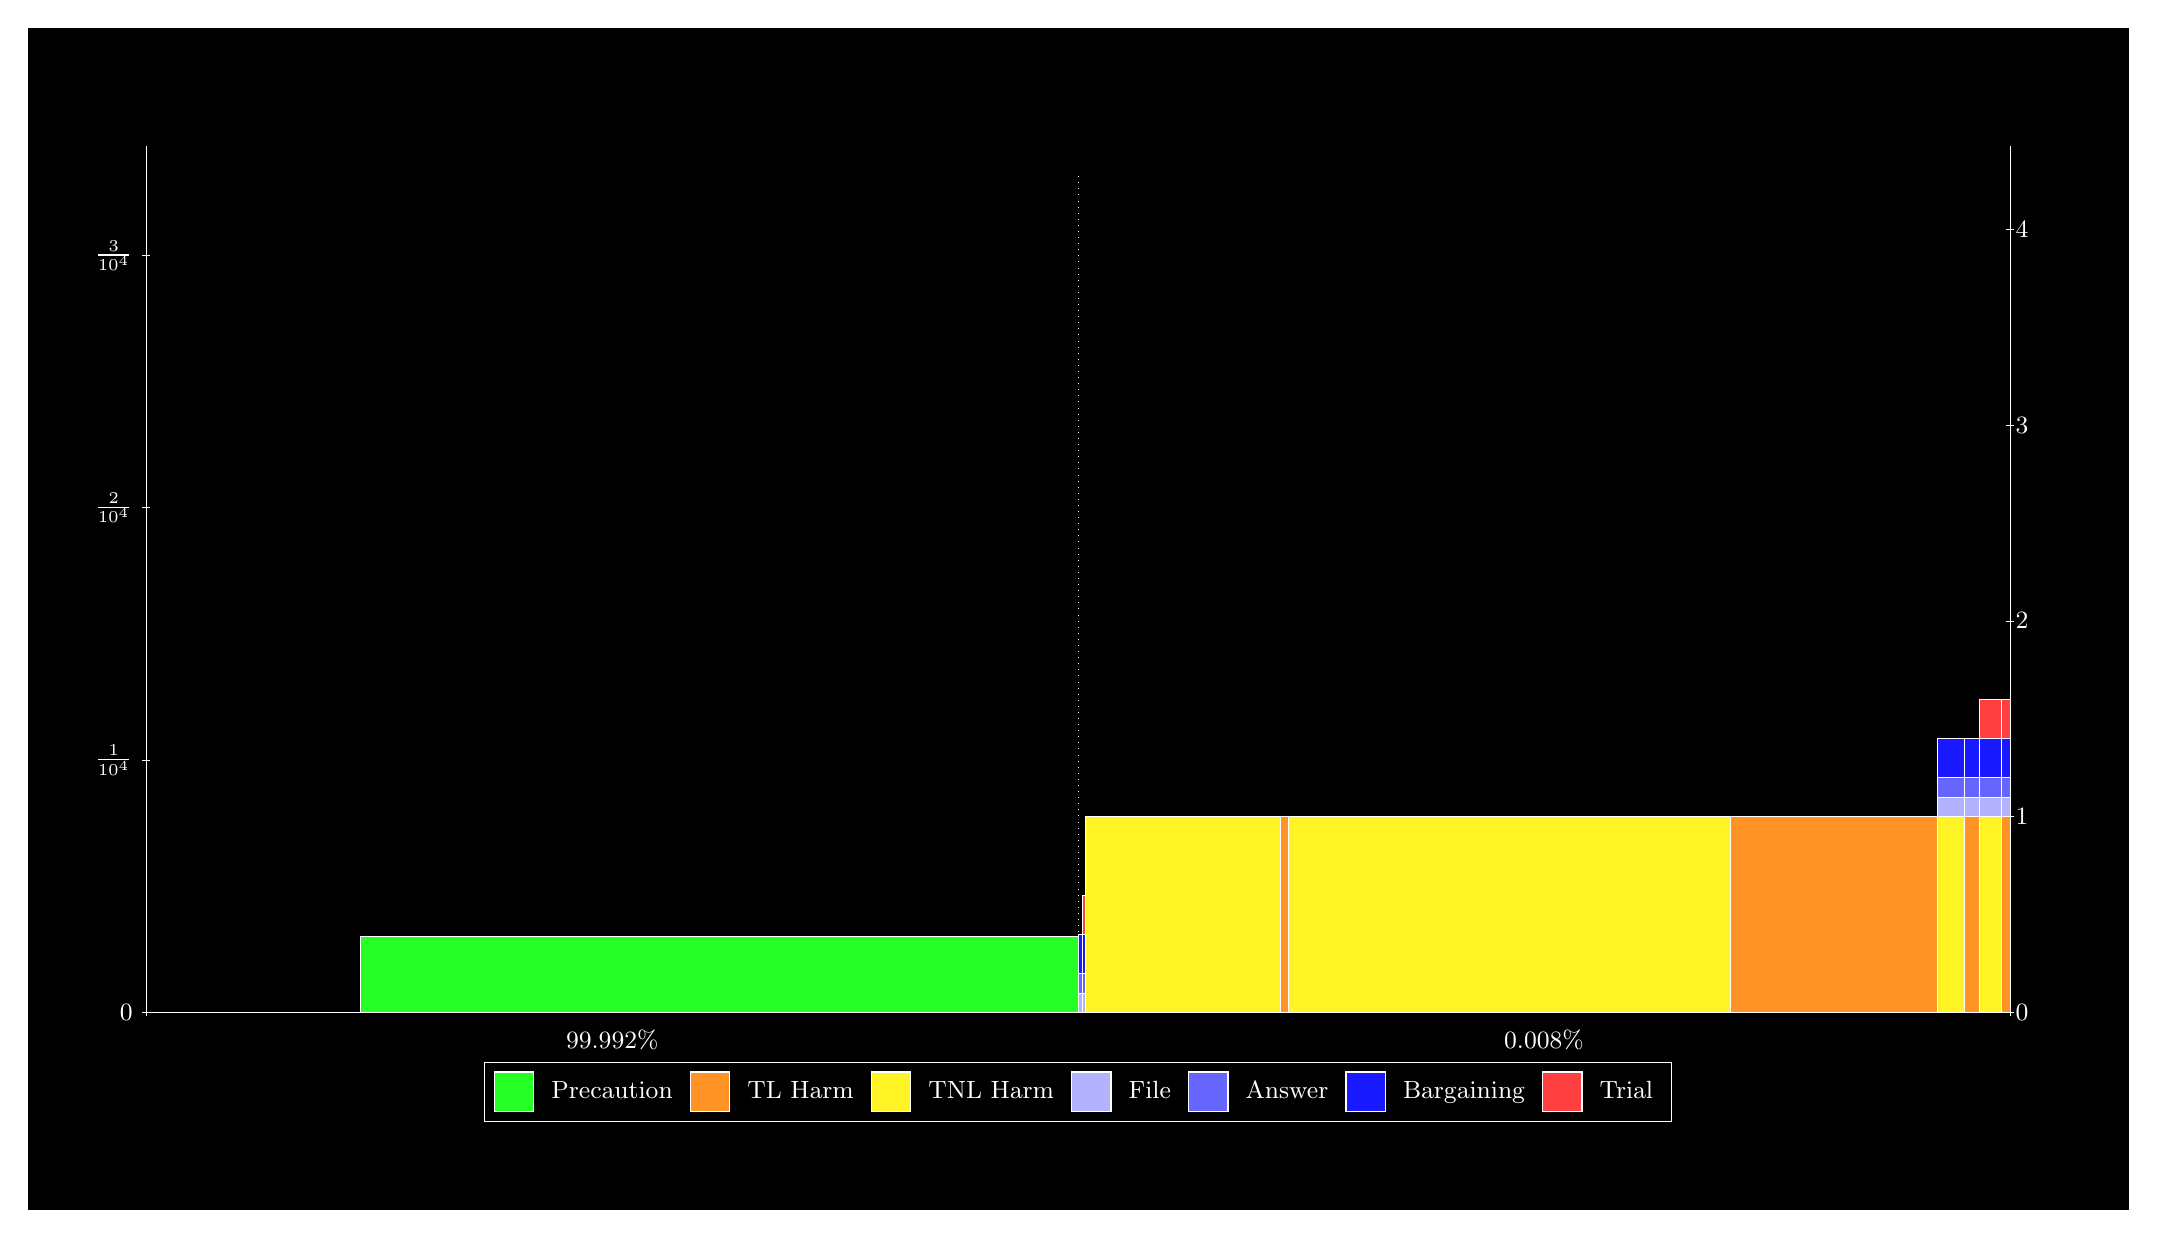
\begin{tikzpicture}
\draw[fill=black] (0,0) rectangle (26.667,15);
\draw[fill=green!85,draw=white,very thin] (4.2218,2.5) rectangle (13.333,3.4616);
\draw[fill=blue!30,draw=white,very thin] (13.333,2.5) rectangle (13.387,2.7487);
\draw[fill=blue!60,draw=white,very thin] (13.333,2.7487) rectangle (13.387,2.9974);
\draw[fill=blue!90,draw=white,very thin] (13.333,2.9974) rectangle (13.387,3.4948);
\draw[fill=blue!30,draw=white,very thin] (13.387,2.5) rectangle (13.426,2.7487);
\draw[fill=blue!60,draw=white,very thin] (13.387,2.7487) rectangle (13.426,2.9974);
\draw[fill=blue!90,draw=white,very thin] (13.387,2.9974) rectangle (13.426,3.4948);
\draw[fill=red!75,draw=white,very thin] (13.387,3.4948) rectangle (13.426,3.9922);
\draw[fill=yellow!85,draw=white,very thin] (13.426,2.5) rectangle (15.895,4.9871);
\draw[fill=orange!85,draw=white,very thin] (15.895,2.5) rectangle (16.007,4.9871);
\draw[fill=green!85,draw=white,very thin] (16.007,2.5) rectangle (21.612,2.5001);
\draw[fill=yellow!85,draw=white,very thin] (16.007,2.5001) rectangle (21.612,4.9871);
\draw[fill=green!85,draw=white,very thin] (21.612,2.5) rectangle (24.24,2.5001);
\draw[fill=orange!85,draw=white,very thin] (21.612,2.5001) rectangle (24.24,4.9871);
\draw[fill=yellow!85,draw=white,very thin] (24.24,2.5) rectangle (24.583,4.9871);
\draw[fill=blue!30,draw=white,very thin] (24.24,4.9871) rectangle (24.583,5.2358);
\draw[fill=blue!60,draw=white,very thin] (24.24,5.2358) rectangle (24.583,5.4845);
\draw[fill=blue!90,draw=white,very thin] (24.24,5.4845) rectangle (24.583,5.9819);
\draw[fill=orange!85,draw=white,very thin] (24.583,2.5) rectangle (24.778,4.9871);
\draw[fill=blue!30,draw=white,very thin] (24.583,4.9871) rectangle (24.778,5.2358);
\draw[fill=blue!60,draw=white,very thin] (24.583,5.2358) rectangle (24.778,5.4845);
\draw[fill=blue!90,draw=white,very thin] (24.583,5.4845) rectangle (24.778,5.9819);
\draw[fill=yellow!85,draw=white,very thin] (24.778,2.5) rectangle (25.055,4.9871);
\draw[fill=blue!30,draw=white,very thin] (24.778,4.9871) rectangle (25.055,5.2358);
\draw[fill=blue!60,draw=white,very thin] (24.778,5.2358) rectangle (25.055,5.4845);
\draw[fill=blue!90,draw=white,very thin] (24.778,5.4845) rectangle (25.055,5.9819);
\draw[fill=red!75,draw=white,very thin] (24.778,5.9819) rectangle (25.055,6.4793);
\draw[fill=orange!85,draw=white,very thin] (25.055,2.5) rectangle (25.167,4.9871);
\draw[fill=blue!30,draw=white,very thin] (25.055,4.9871) rectangle (25.167,5.2358);
\draw[fill=blue!60,draw=white,very thin] (25.055,5.2358) rectangle (25.167,5.4845);
\draw[fill=blue!90,draw=white,very thin] (25.055,5.4845) rectangle (25.167,5.9819);
\draw[fill=red!75,draw=white,very thin] (25.055,5.9819) rectangle (25.167,6.4793);
\draw[white,very thin] (1.5,2.5) -- (1.5,13.5);
\draw[white,very thin] (1.45,2.5) -- (1.55,2.5);
\node[font=\small,text=white, anchor=east] at (1.45, 2.5) {0};
\draw[white,very thin] (1.45,5.7052) -- (1.55,5.7052);
\node[font=\small,text=white, anchor=east] at (1.45, 5.7052) {$\frac{1}{10^{4}}$};
\draw[white,very thin] (1.45,8.9104) -- (1.55,8.9104);
\node[font=\small,text=white, anchor=east] at (1.45, 8.9104) {$\frac{2}{10^{4}}$};
\draw[white,very thin] (1.45,12.116) -- (1.55,12.116);
\node[font=\small,text=white, anchor=east] at (1.45, 12.116) {$\frac{3}{10^{4}}$};

\draw[white,dotted,very thin] (13.333,2.83) -- (13.333,13.17);
\draw[white,very thin] (25.167,2.5) -- (25.167,13.5);
\draw[white,very thin] (25.117,2.5) -- (25.217,2.5);
\node[font=\small,text=white, anchor=west] at (25.117, 2.5) {0};
\draw[white,very thin] (25.117,4.9871) -- (25.217,4.9871);
\node[font=\small,text=white, anchor=west] at (25.117, 4.9871) {1};
\draw[white,very thin] (25.117,7.4741) -- (25.217,7.4741);
\node[font=\small,text=white, anchor=west] at (25.117, 7.4741) {2};
\draw[white,very thin] (25.117,9.9612) -- (25.217,9.9612);
\node[font=\small,text=white, anchor=west] at (25.117, 9.9612) {3};
\draw[white,very thin] (25.117,12.448) -- (25.217,12.448);
\node[font=\small,text=white, anchor=west] at (25.117, 12.448) {4};

\draw[white,very thin] (1.5,2.5) -- (25.167,2.5);
\draw[white,very thin] (1.5,2.45) -- (1.5,2.55);
\node[font=\small,text=white, anchor=north] at (1.5, 2.45) {};
\draw[white,very thin] (25.167,2.45) -- (25.167,2.55);
\node[font=\small,text=white, anchor=north] at (25.167, 2.45) {};

\node[font=\small,text=white,anchor=south] at (7.4167, 1.9) {99.992\%};
\node[font=\small,text=white,anchor=south] at (19.25, 1.9) {0.008\%};
\draw (13.3333,2.5) node (B) {};
\begin{scope}[align=center]
\matrix[scale=0.5,draw=white,below=0.5cm of B,nodes={draw},column sep=0.1cm]{
\node[rectangle,draw,minimum width=0.5cm,minimum height=0.5cm,fill=green!85]{}; & \node[draw=none,font=\small,text=white]{Precaution}; &
\node[rectangle,draw,minimum width=0.5cm,minimum height=0.5cm,fill=orange!85]{}; & \node[draw=none,font=\small,text=white]{TL Harm}; &
\node[rectangle,draw,minimum width=0.5cm,minimum height=0.5cm,fill=yellow!85]{}; & \node[draw=none,font=\small,text=white]{TNL Harm}; &
\node[rectangle,draw,minimum width=0.5cm,minimum height=0.5cm,fill=blue!30]{}; & \node[draw=none,font=\small,text=white]{File}; &
\node[rectangle,draw,minimum width=0.5cm,minimum height=0.5cm,fill=blue!60]{}; & \node[draw=none,font=\small,text=white]{Answer}; &
\node[rectangle,draw,minimum width=0.5cm,minimum height=0.5cm,fill=blue!90]{}; & \node[draw=none,font=\small,text=white]{Bargaining}; &
\node[rectangle,draw,minimum width=0.5cm,minimum height=0.5cm,fill=red!75]{}; & \node[draw=none,font=\small,text=white]{Trial}; \\\\
};\end{scope}

\end{tikzpicture}
\end{document}